\documentclass{jdmdh}
\usepackage[utf8]{inputenc}
\usepackage{array}
\usepackage{pgfplots}

\title{Evaluating Deep Learning Methods for Tokenization of Scripta Continua in Old French and Latin}
\author[1]{Thibault Clérice}
\affil[1]{École nationale des Chartes, France} 
\affil[2]{Université Lyon 3, France} 

\corrauthor{Thibault Clérice}{thibault.clerice@chartes.psl.eu}



\begin{document}

\maketitle

\abstract{Tokenization of modern and old Western European languages seems to be fairly simple as it stands on the presence mostly of markers such as spaces and punctuation. Although, when dealing with old sources like manuscript written in \textit{scripta continua}, (1) such markers are mostly absent, (2) spelling variation and rich morphologies makes dictionary based approaches difficult. We show that a convolutional encoder of characters followed by linear categorization can be used to tokenize such inputs. Additionaly, we release a software with a rather simple interface.}

\keywords{convolutional network; scripta continua; tokenization; Latin; Old French}

\section{Introduction}

\strut
\vspace{-4ex}

Sed eu tempor ipsum, vel cursus arcu. Maecenas non dignissim nunc, ac ornare tortor. Aenean
pretium arcu metus, id pulvinar enim tempus nec. Mauris faucibus mollis sodales. Sed
porttitor sed metus vitae vestibulum. Quisque a vehicula nunc. Aenean fringilla condimentum
diam, ac gravida quam. Integer ultrices feugiat enim nec tempus. Vestibulum ornare in magna
ultrices dapibus. Nulla facilisi. 

\section{Title}

\subsection{Subtitle}
Pellentesque dignissim ultrices fringilla. Vivamus eu luctus ante, vel bibendum magna.
Curabitur elit purus, tincidunt non dui vitae, elementum bibendum neque. Curabitur
ullamcorper sit amet justo at hendrerit. Fusce ut arcu imperdiet nibh mollis tempus a aliquet
tellus. Quisque pharetra cursus nisi, vel lobortis ante consectetur et. Vivamus sed congue
neque. Proin pellentesque risus nec dui consequat rutrum. Vestibulum nunc diam, placerat
quis auctor vel, faucibus non justo. Etiam dictum purus neque. Phasellus imperdiet mauris
ligula, eu laoreet nisi elementum ut. Sed sed porta massa. Aenean faucibus risus ultrices
ornare porta. Quisque faucibus ante a tincidunt vestibulum. Lorem ipsum dolor sit amet,
consectetur adipiscing elit.


\subsubsection{Sub-subtitle}
Suspendisse vel dui nec felis molestie tincidunt. Vestibulum rutrum ligula lacus, ac molestie
nulla fermentum ornare. Nulla non nunc euismod, porta lacus vestibulum, malesuada massa.
Curabitur massa eros, rutrum sed lectus sed, volutpat semper metus. Mauris hendrerit aliquam
commodo.  Vivamus fermentum tempus pellentesque. Maecenas a hendrerit urna. In elit
ipsum, ultrices non dolor in, pulvinar porttitor lacus. Nunc euismod nibh quis odio
condimentum, a feugiat massa rutrum. Nulla erat erat, adipiscing vitae lectus id, consectetur
fermentum elit. Nunc eu est eu neque dapibus semper. Nam commodo urna dapibus, tincidunt
turpis a, cursus sem. Vivamus venenatis adipiscing mollis. Cras fringilla sodales lobortis.
Aliquam aliquet felis id est cursus auctor. Duis sodales tellus vulputate lectus egestas
volutpat.


\section{Tables and Figures}

\subsection{Table}
see Table~\ref{tab:example}.

\begin{table}
  \newcolumntype{+}{>{\global\let\currentrowstyle\relax}}
  \newcolumntype{^}{>{\currentrowstyle}}
  \newcommand{\rowstyle}[1]{\gdef\currentrowstyle{#1}%
    #1\ignorespaces
  }

  \centering
  \begin{tabular}{+>{\bfseries}l^c^c^c^c}
    \hline
    \rowstyle{\bfseries}
    & Sepal.Length & Sepal.Width & Petal.Length & Petal.Width\\
    Setosa & 5.006 & 3.428 & 1.462 & 0.246\\
    Versicolor & 5.936 & 2.77  & 4.26  & 1.326\\
    Verginica & 6.588 & 2.974 & 5.552 & 2.026\\
    \hline
  \end{tabular}

  \caption{Morbi malesuada diam at magna condimentum.}
  \label{tab:example}
\end{table}


\subsection{Figure}

Use subfigures to group similar images into one figure. Make pictures with a good resolution, as possible closed to 300 dpi or use vector graphics as for example provided by the TikZ package. Ensure that all legends are readable and in English. See example in Figure~\ref{fig:example} (taken from \url{http://www.texample.net/tikz/examples/pgfplots/}).


\begin{figure}
  \centering
  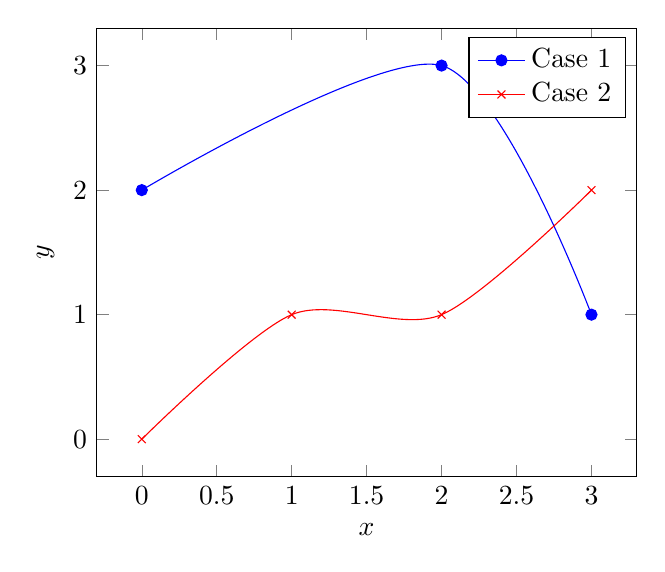
\begin{tikzpicture}
    \begin{axis}[
        xlabel=$x$,
        ylabel=$y$]
    \addplot[smooth,mark=*,blue] plot coordinates {
        (0,2)
        (2,3)
        (3,1)
    };
    \addlegendentry{Case 1}

    \addplot[smooth,color=red,mark=x]
        plot coordinates {
            (0,0)
            (1,1)
            (2,1)
            (3,2)
        };
    \addlegendentry{Case 2}
    \end{axis}
    \end{tikzpicture}

  \caption{Figure by Christian Feuers\"anger; Source: Pgfplots manual}
  \label{fig:example}
\end{figure}

\section{Definitions, Algorithms, and Formulas}

\subsection{Definitions}
You can define your own environments for formulas with the methods of the \texttt{amsthm} package. Use the theoremstyle \texttt{jdmdh} for a consistent formatting.

\begin{definition}[alpha]
Curabitur ullamcorper sit amet justo at hendrerit.
\end{definition}

Hence we set the following definition:

\begin{definition}
Etiam sed nulla viverra, ultrices ligula ac, consectetur libero.
\end{definition}


If you used a list, you need to write a bullet list:
\begin{itemize}
  \item Nunc id justo scelerisque.
  \item metus id enim iaculis tristique.
\end{itemize}

\subsection{Formulas}

Example of formula:
\begin{equation}
  Y=M.^tM-\beta.\langle M \rangle_l
\end{equation}

where $\langle M \rangle_l$ is a mean vector of a line from $M$. $\beta$ plays as a regulation factor to regulate the
rate of nearest neighbours, in fact the number of nearest neighbours is not defined explicitly.

Another example of a formula:
\begin{equation}
  K * N_c = Cst \pm 0.001\%
\end{equation}

\subsection{Algorithms}

This is a short algorithm:
\begin{lstlisting}[numbers=none]
quicksort(A, i, k):
  if i < k:
    p := partition(A, i, k)
    quicksort(A, i, p - 1)
    quicksort(A, p + 1, k)
\end{lstlisting}

For longer algorithms, use a float environment as shown in Listing~\ref{lst:example}. For configurations to specific languages, see the reference manual of the \texttt{listings} package.

\begin{listing}
  \begin{lstlisting}
  partition(array, left, right)
     pivotIndex := choose-pivot(array, left, right)
     pivotValue := array[pivotIndex]
     swap array[pivotIndex] and array[right]
     storeIndex := left
     for i from left to right - 1
         if array[i] < pivotValue
             swap array[i] and array[storeIndex]
             storeIndex := storeIndex + 1
     swap array[storeIndex] and array[right]  // Move pivot to its final place
     return storeIndex
  \end{lstlisting}

  \caption{Partition function of quicksort algorithm.}
  \label{lst:example}
\end{listing}



\section{References and Citations}
From \citet{sinclair91corpus} we pick up a general definition ...\\
\citet{ounis00flidar} explain that ...\\
\citet{wood92artifacts} recommend ...

% The \nocite command here is only intended to show more examples of references; please only list works that you really reference in your article
\nocite{hentschel07acceptance,biodiversa,pubmed,antonymy02perspective,justeson01cooccurence,r-project}

\subsection{Discussion}
Nam id eros massa. Fusce luctus purus a augue ullamcorper, sit amet vehicula mauris
tristique. Suspendisse eget pulvinar odio, nec bibendum turpis. Nullam quis lectus porttitor,
ullamcorper nisi et, condimentum leo. Quisque sed orci fermentum, rutrum velit eget, ultricies
augue. Nunc porttitor consectetur tincidunt. Nulla tincidunt justo enim, vitae dignissim erat
mattis ut. Nulla.

\subsection{Conclusion}
Maecenas egestas metus id enim iaculis tristique. Etiam sed nulla viverra, ultrices ligula ac,
consectetur libero. Nullam vitae massa ac odio pharetra condimentum. Maecenas in
elementum libero, non gravida quam. Praesent adipiscing consectetur consectetur. Vivamus at
orci sed augue varius hendrerit. Donec neque metus, dignissim nec erat at, ultricies consequat
libero. Donec eget eleifend leo. Aliquam at nunc porta, mollis sapien eu, eleifend tortor. Nam
egestas, metus ac pellentesque feugiat, lectus purus ornare est, vitae cursus felis turpis sit amet
lacus. Donec consequat massa mi, ac suscipit arcu posuere et. Vivamus et semper risus. Sed ut
arcu quam.


\bibliographystyle{plainnat}
\bibliography{jdmdh-example}

\appendix\footnotesize

\section{Annex 1}
Pellentesque dignissim ultrices fringilla. Vivamus eu luctus ante, vel bibendum magna. Curabitur elit purus, tincidunt non dui
vitae, elementum bibendum neque. Curabitur ullamcorper sit amet justo at hendrerit. Fusce ut arcu imperdiet nibh mollis
tempus a aliquet tellus. Quisque pharetra cursus nisi, vel lobortis ante consectetur et. Vivamus sed congue neque. Proin
pellentesque risus nec dui consequat rutrum. Vestibulum nunc diam, placerat quis auctor vel, faucibus non justo. Etiam
dictum purus neque. Phasellus imperdiet mauris ligula, eu laoreet nisi elementum ut. Sed sed porta massa. Aenean faucibus
risus ultrices ornare porta. Quisque faucibus ante a tincidunt vestibulum. Lorem ipsum dolor sit amet, consectetur adipiscing
elit.


\section{Annex 2}
Cras tristique vel nisi at aliquet. Proin egestas erat sit amet velit lobortis imperdiet. Integer et arcu sapien. Etiam id blandit
sapien. Nam tempus lacus ac massa semper, vel laoreet turpis rutrum. Mauris eget nibh vitae justo porta imperdiet sed vel
ligula. In imperdiet, augue vel condimentum convallis, neque augue imperdiet neque, eget dapibus nunc mauris ultricies
tortor. Nam eget nunc egestas, blandit lectus non, aliquam nunc. Cras sed quam vitae arcu ornare lobortis. Ut ut lacus
hendrerit, convallis orci sit amet, commodo nunc. Pellentesque eget tincidunt tortor. Nunc ornare molestie mauris id vehicula.
Suspendisse pharetra tortor metus, sit amet fermentum tellus vehicula ut.


\end{document}